% Gaussstrahlen

\section{Gaußstrahlen}
\label{sec:gauss}

\subsection{Strahlausbreitungsparameter $M^2$}

\subsubsection*{ohne Fernfeldnäherung}

Für die Breite eines idealen Gaußstrahls gilt laut Skript 
\begin{equation*}
    w_G(z) = w_{0,G} \sqrt{1 + \biggl(\frac{\lambda z}{\pi w_{0,G}^2}\biggl)^2}.
\end{equation*}

Damit ergibt sich für den Stahldurchmesser 
\begin{equation*}
    d_G(z) = 2 w_G(z) = 2 w_{0,G} \sqrt{1 + \biggl(\frac{\lambda z}{\pi w_{0,G}^2}\biggl)^2} = d_{0,G} \sqrt{1 + \biggl(\frac{4\lambda z}{\pi d_{0,G}^2}\biggl)^2}.
\end{equation*}

Weicht der Strahl nun von einem idealen Gaußstrahl ab, so wird sein Durchmesser um den Faktor $M$ größer. Er berechnet sich nach
\begin{equation*}
    d(z) = M d_{0,G} \sqrt{1 + \biggl(\frac{4\lambda z}{\pi d_{0,G}^2}\biggl)^2} = d_0 \sqrt{1 +\biggl (\frac{4M^2\lambda z}{\pi d_0^2}\biggl)^2},
\end{equation*}
wobei $d_0$ hier der Durchmesser der Strahltallie des nicht-idealen Gaußstrahls ist.
Für einen Abstand $z = -(L_2-L_1)/2$ ergibt sich also
\begin{align}
    d_1 &= d(-(L_2-L_1)/2) = d_0 \sqrt{1 +\biggl (\frac{-(L_2-L_1)2M^2\lambda}{\pi d_0^2}\biggl)^2} \nonumber \\
    \leftrightarrow M^2 &= \frac{\pi d_0^2}{2 \lambda (L_2-L_1) } \sqrt{\biggl(\frac{d_1}{d_0}\biggl)^2-1},
    \label{eq:M}
\end{align}
was die Formel zur Berechnung des Strahlausbreitungsparameters aus dem Skript ist.

Im Folgenden soll mithilfe dieser Formel der Strahlausbreitungsparameter für den Experimentier- und den Hilfslaser bestimmt werden. Dazu wurde die Intensität der Strahlen 
nach dem Durchgang durch eine Linse (f = 300\,$\frac{1}{m}$) an verschiedenen Positionen mit einer CCD-Kamera gemessen. Dabei wurden die Daten entlang einer horizontalen und 
einer vertikalen Achse durch den Bereich des Strahlquerschnitts mit der höchsten Intensität entnommen. Nachdem eine gaußförmige Verteilung der Intensität erwartet wird, wird 
eine Funktion der Form 
\begin{equation*}
    I(x) = I_0 \exp(\frac{-2(x-x_0)^2}{w^2}) + I_{off}
\end{equation*}

an die Datensätze gefittet. Der Parameter $I_{off}$ ist durch den Offset in den gemessenen Intensitäten der Kamera bedingt. Aus diesen Fits ergeben sich die Breiten und Fehler der 
Strahlen $w$, die in Tab.\ref{tab:M} bis \ref{tab:M3} zu sehen sind. Für Berechnungen, die die Strahldurchmesser $d$ benötigen, müssen die Werte von $w$ und $s_w$ einfach verdoppelt werden.
%TABELLE

\begin{table}
    \centering
    \begin{tabular}{rrrrrr}
        \toprule
        $L$ / mm &  $s_L$ / mm &    $w$ / mm &  $s_w$ / mm&     $M^2$ &        $s_M^2$ \\
        \midrule
        770 &  10 &  0,05928 &  0,00042 &        &        \\
        780 &  10 &  0,06022 &  0,00028 &  0,312 &  0,449 \\
        760 &  10 &  0,07365 &  0,00070 &  1,286 &  1,819 \\
        790 &  10 &  0,08248 &  0,00043 &  0,844 &  0,596 \\
        750 &  10 &  0,09498 &  0,00084 &  1,092 &  0,772 \\
        800 &  10 &  0,11303 &  0,00047 &  0,944 &  0,445 \\
        740 &  10 &  0,12093 &  0,00045 &  1,034 &  0,487 \\
        730 &  10 &  0,14284 &  0,00062 &  0,956 &  0,338 \\
        810 &  10 &  0,15814 &  0,00067 &  1,078 &  0,381 \\
        720 &  10 &  0,17334 &  0,00058 &  0,958 &  0,271 \\
        820 &  10 &  0,19323 &  0,00112 &  1,082 &  0,306 \\
        700 &  10 &  0,22388 &  0,00110 &  0,907 &  0,183 \\
        840 &  10 &  0,25699 &  0,00111 &  1,051 &  0,212 \\
        680 &  10 &  0,31518 &  0,00152 &  1,012 &  0,159 \\
        860 &  10 &  0,33974 &  0,00162 &  1,093 &  0,172\\
        660 &  10 &  0,36696 &  0,00205 &  0,968 &  0,124 \\
        880 &  10 &  0,38290 &  0,00232 &  1,012 &  0,130 \\
        600 &  10 &  0,55240 &  0,00250 &  0,950 &  0,079 \\
        960 &  10 &  0,61462 &  0,00377 &  0,947 &  0,071 \\
        500 &  10 &  0,91721 &  0,01036 &  0,997 &  0,053 \\
        \bottomrule
    \end{tabular}
    \captionof{table}{Werte der verschiedenen Strahlbreiten $w$, Strahlausbreitungsparameter $M^2$ und zugehörige Fehler für verschiedene Positionen $L$ 
    des horizontalen Schnitts durch den Strahl des Experimentierlasers. Die Werte sind aufsteigend nach $w$ sortiert. Der Wert für $L$ = 770\,mm wurde als Strahltaille benutzt; deshalb existieren 
    hier keine Werte für $M^2$ und dessen Fehler.}
    \label{tab:M}
\end{table}

\begin{table}
    \centering
    \begin{tabular}{rrrrrr}
        \toprule
        $L$ / mm&  $s_L$ / mm &      $w$ / mm&    $s_w$ / mm&         $M^2$ &        $s_M^2$ \\
        \midrule
        780 &  10 &  0,0609 &  0,0002 &       &       \\
        770 &  10 &  0,0614 &  0,0004 &  0,22 &  0,33 \\
        760 &  10 &  0,0775 &  0,0007 &  0,72 &  0,51 \\
        790 &  10 &  0,0800 &  0,0004 &  1,57 &  2,22 \\
        750 &  10 &  0,0992 &  0,0008 &  0,79 &  0,37 \\
        800 &  10 &  0,1076 &  0,0004 &  1,34 &  0,94 \\
        740 &  10 &  0,1288 &  0,0004 &  0,85 &  0,30 \\
        730 &  10 &  0,1524 &  0,0006 &  0,84 &  0,23 \\
        810 &  10 &  0,1548 &  0,0005 &  1,43 &  0,67 \\
        720 &  10 &  0,1825 &  0,0006 &  0,86 &  0,20 \\
        820 &  10 &  0,1885 &  0,0009 &  1,35 &  0,47 \\
        700 &  10 &  0,2301 &  0,0012 &  0,83 &  0,14 \\
        840 &  10 &  0,2503 &  0,0010 &  1,22 &  0,28 \\
        860 &  10 &  0,3015 &  0,0013 &  1,11 &  0,19 \\
        680 &  10 &  0,3178 &  0,0013 &  0,94 &  0,13 \\
        880 &  10 &  0,3737 &  0,0019 &  1,11 &  0,15 \\
        660 &  10 &  0,3869 &  0,0025 &  0,96 &  0,11 \\
        600 &  10 &  0,5885 &  0,0040 &  0,98 &  0,07 \\
        960 &  10 &  0,6066 &  0,0049 &  1,01 &  0,08 \\
        500 &  10 &  0,9058 &  0,0105 &  0,97 &  0,05 \\
        \bottomrule
    \end{tabular}
    \captionof{table}{Werte der verschiedenen Strahlbreiten $w$, Strahlausbreitungsparameter $M^2$ und zugehörige Fehler für verschiedene Positionen $L$ 
    des vertikalen Schnitts durch den Strahl des Experimentierlasers. Die Werte sind aufsteigend nach $w$ sortiert. Der Wert für $L$ = 780\,mm wurde als Strahltaille benutzt; deshalb existieren 
    hier keine Werte für $M^2$ und dessen Fehler.}
    \label{tab:M1}
\end{table}

\begin{table}
    \centering
    \begin{tabular}{rrrrrr}
        \toprule
        $L$ / mm &  $s_L$ / mm &    $w$ / mm &  $s_w$ / mm&     $M^2$ &        $s_M^2$ \\
        \midrule
        830 &  10 &  0,0583 &  0,0006 &       &      \\
        820 &  10 &  0,0619 &  0,0005 &  0,60 &  0,85 \\
        810 &  10 &  0,0710 &  0,0006 &  0,58 &  0,41 \\
        840 &  10 &  0,1022 &  0,0010 &  2,43 &  3,43 \\
        800 &  10 &  0,1047 &  0,0010 &  0,83 &  0,39 \\
        850 &  10 &  0,1320 &  0,0012 &  1,71 &  1,21 \\
        790 &  10 &  0,1428 &  0,0011 &  0,94 &  0,33 \\
        780 &  10 &  0,1747 &  0,0010 &  0,95 &  0,26 \\
        860 &  10 &  0,1780 &  0,0015 &  1,62 &  0,76 \\
        870 &  10 &  0,2169 &  0,0016 &  1,51 &  0,53 \\
        770 &  10 &  0,2235 &  0,0015 &  1,04 &  0,24 \\
        760 &  10 &  0,2646 &  0,0015 &  1,06 &  0,21 \\
        890 &  10 &  0,3102 &  0,0025 &  1,47 &  0,34 \\
        740 &  10 &  0,3410 &  0,0028 &  1,08 &  0,17 \\
        910 &  10 &  0,3875 &  0,0030 &  1,38 &  0,24 \\
        720 &  10 &  0,4217 &  0,0025 &  1,09 &  0,14 \\
        930 &  10 &  0,4578 &  0,0034 &  1,31 &  0,18 \\
        700 &  10 &  0,5104 &  0,0038 &  1,12 &  0,12 \\
        950 &  10 &  0,5229 &  0,0056 &  1,25 &  0,14 \\
        650 &  10 &  0,6915 &  0,0074 &  1,10 &  0,08 \\
        550 &  10 &  1,1528 &  0,0174 &  1,19 &  0,06 \\
        \bottomrule
    \end{tabular}
    \captionof{table}{Werte der verschiedenen Strahlbreiten $w$, Strahlausbreitungsparameter $M^2$ und zugehörige Fehler für verschiedene Positionen $L$ 
    des horizontalen Schnitts durch den Strahl des Hilfslasers. Die Werte sind aufsteigend nach $w$ sortiert. Der Wert für $L$ = 770\,mm wurde als Strahltaille benutzt; deshalb existieren 
    hier keine Werte für $M^2$ und dessen Fehler.}
    \label{tab:M2}
\end{table}

\begin{table}
    \centering
    \begin{tabular}{rrrrrr}
        \toprule
        $L$ / mm &  $s_L$ / mm &    $w$ / mm &  $s_w$ / mm&     $M^2$ &        $s_M^2$ \\
        \midrule
        820 &  10 &  0,0622 &  0,00047 &       &       \\
        810 &  10 &  0,0663 &  0,0003 &  0,70 &  1,00 \\
        830 &  10 &  0,0686 &  0,0006 &  0,89 &  1,26 \\
        800 &  10 &  0,0816 &  0,0008 &  0,81 &  0,57 \\
        840 &  10 &  0,0982 &  0,0008 &  1,17 &  0,83 \\
        790 &  10 &  0,1106 &  0,0008 &  0,94 &  0,44 \\
        850 &  10 &  0,1301 &  0,0009 &  1,17 &  0,55 \\
        780 &  10 &  0,1494 &  0,0008 &  1,04 &  0,37 \\
        860 &  10 &  0,1699 &  0,0008 &  1,22 &  0,43 \\
        770 &  10 &  0,1771 &  0,0011 &  1,02 &  0,29 \\
        870 &  10 &  0,2021 &  0,0009 &  1,18 &  0,33 \\
        760 &  10 &  0,2078 &  0,0010 &  1,02 &  0,24 \\
        740 &  10 &  0,2639 &  0,0009 &  0,99 &  0,17 \\
        890 &  10 &  0,2657 &  0,0010 &  1,14 &  0,23 \\
        720 &  10 &  0,3357 &  0,0016 &  1,01 &  0,14 \\
        910 &  10 &  0,3361 &  0,0015 &  1,13 &  0,17 \\
        700 &  10 &  0,4155 &  0,0027 &  1,05 &  0,12 \\
        930 &  10 &  0,4250 &  0,0024 &  1,18 &  0,15 \\
        950 &  10 &  0,4556 &  0,0022 &  1,07 &  0,11 \\
        650 &  10 &  0,5865 &  0,0037 &  1,06 &  0,08 \\
        550 &  10 &  0,9381 &  0,0128 &  1,07 &  0,05 \\
        \bottomrule
    \end{tabular}
    \captionof{table}{Werte der verschiedenen Strahlbreiten $w$, Strahlausbreitungsparameter $M^2$ und zugehörige Fehler für verschiedene Positionen $L$ 
    des vertikalen Schnitts durch den Strahl des Hilfslasers. Die Werte sind aufsteigend nach $w$ sortiert. Der Wert für $L$ = 770\,mm wurde als Strahltaille benutzt; deshalb existieren 
    hier keine Werte für $M^2$ und dessen Fehler.}
    \label{tab:M3}
\end{table}

Zur Berechnung des Strahlausbreitungsparameters wird Gl.\ref{eq:M} umgeschrieben zu
\begin{equation*}
    M^2 = \frac{\pi d_0^2}{2 \lambda 2|L_0-L_1| } \sqrt{\biggl(\frac{d_1}{d_0}\biggl)^2-1},
\end{equation*}
wobei verwendet wurde, dass $d_1$ und $d_2$ symmetrisch um $d_0$ liegen.\\
Für $d_0$ (und $L_0$) werden jeweils die kleinsten Werte der Strahldurchmesser der jeweiligen Messreihen gewählt und $M^2$ für alle anderen Werte von $d$ (und $L$) als 
$d_1$ ($L_1$) berechnet. Der Fehler für $M^2$ ergibt sich aus der klassischen Fehlerfortpflanzung unter der Verwendung folgender partieller Ableitungen:
\begin{align*}
    \partial_{d_0}M^2 &= \frac{M^2}{d_0}(2-\frac{1}{1-(\frac{d_0}{d_1})^2}) \\
    \partial_{d_1}M^2 &= \frac{M^2}{d_1 - \frac{d_0^2}{d_1}} \\
    \partial_{L_{0/1}}M^2 &= \pm \frac{M^2}{L_0-L_1} \\
\end{align*}
Dabei wurde für die Längen ein Fehler von 10\,mm angenommen, da die Position der Kamera auf ihrem Schlitten nicht eindeutig festzustellen war. 
Die berechneten $M^2$ mit zugehörigen Fehlern $s_{M^2}$ finden sich ebenfalls in Tab.\ref{tab:M} bis \ref{tab:M3}.
Es ist zu sehen, dass nicht alle Werte von $M^2$ sinnvoll sind. Generell sollten keine Werte kleiner als 1 zu finden sein; davon gibt es unseren Berechnungen nach aber einige. 
Gerade an den Punkten nah an der angenommenen Stahltaille, vor allem beim Experimentierlaser, ist die Abweichung enorm. Dies könnte auch daran liegen, dass die Taille nicht genau getroffen wurde. Um eine Übersicht 
über den Strahlausbreitungsparameter zu erhalten, wird für jede Messreihe der Mittelwert und der dazugehörige Fehler gebildet, wobei die grob abweichenden Werte nah der Taille für den 
Experimentierlaser verworfen werden. Die Ergebnisse sind 
\begin{equation*}
    \textcolor{red}{M^2_{v,exp} = (1,05 \pm 0,15)\,\mathrm{mm}} , \,\, \textcolor{red}{ M^2_{h,exp} = (1,01 \pm 0,14)\,\mathrm{mm}},\\
\end{equation*}
\begin{equation*}
    \textcolor{red}{M^2_{v,hilf} = (1,05 \pm 0,14)\,\mathrm{mm}}\,\,\mathrm{und}\,\,\textcolor{red}{ M^2_{h,hilf} = (1,22 \pm 0,16)\,\mathrm{mm}}.\\    
\end{equation*}
Alle Mittelwerte sind immerhin größer als 1, wenn auch wohl betragsmäßig deutlich zu nah. 
Die Fehler würden zwar geringfügig höhere Werte zulassen; dennoch sind die Werte unseres Erachtens aufgrund methodischer Mängel mit Vorischt zu genießen. Zumindest die 
Größenordnung ist allerdings sinnvoll.

\subsubsection*{Fernfeldmethode}
Eine weitere Möglichkeit zur Bestimmung von $M^2$ ist die Fernfeldmethode. Dabei wird ausgenutzt, dass für $z>5z_R$ (mit Rayleighbereich $z_R$) der Strahlradius sich asymptotisch 
einem Grenzwinkel $\theta_0$ annähert; der Graph des Strahlradius aufgetragen gegen die Postion wird also eine Gerade. 
Die Bereiche, ab denen die Fernfeldnäherung zulässig ist, $5z_R$ ergeben sich nach 
\begin{equation*}
    5z_R = 5 \frac{\pi w_0^2}{\lambda}.
\end{equation*}
Für $w_0$ wurden die selben Taillen wie in der Berechnung ohne Fernfeldnäherung benutzt (vgl. Tab.\ref{tab:M} bis \ref{tab:M3}). Die berechneten Bereiche sind  
\begin{equation*}
    5z_{R,v} = 93,59\,\mathrm{mm} \quad \mathrm{ und } \quad 5z_{R,h} = 87,24\,\mathrm{mm}.
\end{equation*}
In den entsprechenden Bereichen werden nun Geraden gefittet, wie in den Abb.\ref{pic:gerfitve} bis \ref{pic:gerfithh} zu sehen. Aus der Steigung der Geraden ergibt sich $\theta_0$ 
aus 
\begin{equation*}
    \theta_0 = |\arctan(m)|,
\end{equation*}
mit zugehörigem Fehler
\begin{equation*}
    s_{\theta_0} = \frac{1}{1+m^2}s_m,
\end{equation*}
wobei $s_m$ der Fehler aus der linearen Regression ist.
Der Strahlausbreitungsparameter ergibt sich dann aus
\begin{equation*}
    M^2 = \frac{w_0\theta_0 \pi }{\lambda}.
\end{equation*}
Der zughörige Fehler ergibt sich aus der Fehlerfortpflanzung. Die berechneten Werte für $M^2$ und seine Fehler finden sich in Tab.\ref{tab:Mfern}, wobei für jede Messreihe 
zwei Werte berechnet wurden, da die Öffnungswinkel links und rechts der Strahltaille gesondert betrachtet wurden. %tabelle
\begin{table}
    \centering
    \begin{tabular}{rll}
        \toprule
        Wertebereich & Laser & $M^2$ / mm \\
        \midrule
        vertikaler Schnitt, links von Strahltaille & Exp & 0,99 $\pm$ 0,02 \\
        vertikaler Schnitt, rechts von Strahltaille & Exp & 0,887 $\pm$ 0,006 \\
        horizontaler Schnitt, links von Strahltaille & Exp & 0,99 $\pm$ 0,04 \\
        horizontaler Schnitt, rechts von Strahltaille & Exp & 0,82 $\pm$ 0,04 \\
        vertikaler Schnitt, links von Strahltaille & Hilf & 1,088 $\pm$ 0,019 \\
        vertikaler Schnitt, rechts von Strahltaille & Hilf & 0,473 $\pm$ 0,003 \\
        horizontaler Schnitt, links von Strahltaille & Hilf & 1,31 $\pm$ 0,06 \\
        horizontaler Schnitt, rechts von Strahltaille & Hilf & 1,04 $\pm$ 0,03 \\
        \bottomrule
    \end{tabular}
    \captionof{table}{Berechnete Werte für $M^2$ nach der Fernfeldmethode. 'Exp' steht für den Experimentierlaser, 'Hilf' für den Hilfslaser. Dabei sind für den Experimentierlaser sämtliche Werte kleiner als 1, was nicht sein sollte. Der Fehler für den Wert des 
    vertikalen Schnitts rechts von der Strahltaille ist bei beiden Lasern sehr klein; dies liegt daran, dass die Regression selber keinen Fehler hat, da nur zwei Punkte verwendet wurden. Das Ergebnis für den Hilfslaser weicht zudem stark ab, 
    ist deshalb nicht ganz aussagekräftig und wird im weiteren Verlauf auch ausgesondert werden.}
    \label{tab:Mfern}
\end{table}
Dabei ist auch hier festzustellen, dass die Werte zwar in der richtigen Größenordnung liegen. Jedoch sind die Werte, vor allem die des Experimentierlasers deutlich zu klein. 
Die Werte für den Hilfslaser sind etwas besser, abgesehen von dem Wert für den vertikalen Schnitt, rechts von der Taille; dieser wurde allerdings nur über zwei Punkte berechnet, 
die auch anhand der Abb.\ref{pic:gerfitve} bis \ref{pic:gerfithh} als nicht repräsentativ eingeschätzt werden und der Wert für $M^2$ somit übergangen werden kann. Die übrigen Werte scheinen auch 
etwas niedrig, da sie aber größer als 1 sind, sind sie zumindest nicht eindeuig als falsch zu identifizeren. 

\begin{figure}[h]
    \centering
    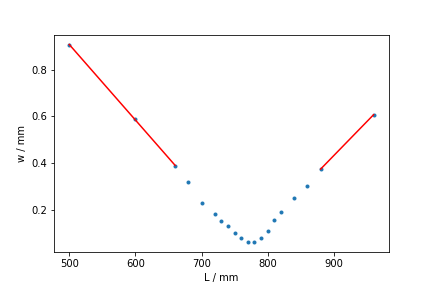
\includegraphics[scale = 0.75]{Bilder/Auswertung/gerfitv.png}
    \caption{Strahldurchmesser $w$ aufgetragen in blauen Punkten gegen die Position $L$ für den vertikalen Schnitt durch den Strahl. Dabei ist der lineare Verlauf für Werte weit entgernt von der Strahltaille 
    gut zu erkennen; die zugehörige lineare Regression ist in Rot eingetragen. Die Regression zur Rechten basiert nur auf zwei Punkten, passt aber dem Augenschein nach trotzdem in etwa zum Verlauf und wird deshalb nicht verworfen.}
    \label{pic:gerfitve}
\end{figure}

\begin{figure}[h]
    \centering
    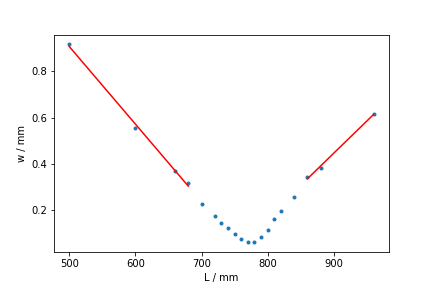
\includegraphics[scale = 0.75]{Bilder/Auswertung/gerfith.png}
    \caption{Strahldurchmesser $w$ aufgetragen in blauen Punkten gegen die Position $L$ für den vertikalen Schnitt durch den Strahl. Dabei ist der lineare Verlauf für Werte weit entgernt von der Strahltaille 
    gut zu erkennen; die zugehörige lineare Regression ist in Rot eingetragen.}
    \label{pic:gerfithe}
\end{figure}

\begin{figure}[h]
    \centering
    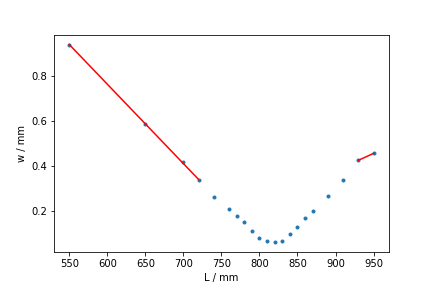
\includegraphics[scale = 0.75]{Bilder/Auswertung/gerfitvh.png}
    \caption{Strahldurchmesser $w$ aufgetragen in blauen Punkten gegen die Position $L$ für den vertikalen Schnitt durch den Strahl. Dabei ist der lineare Verlauf für Werte weit entgernt von der Strahltaille 
    gut zu erkennen; die zugehörige lineare Regression ist in Rot eingetragen. Die Regression zur Rechten basiert nur auf zwei Punkten und ist deshalb von großer Unsicherheit. Da sie zudem augenscheinlich auch 
    nicht die Weiterführung des Graphen ist, kann der aus dieser Geraden resultierende Strahlausbreitungsparameter verworfen werden.}
    \label{pic:gerfitvh}
\end{figure}

\begin{figure}[h]
    \centering
    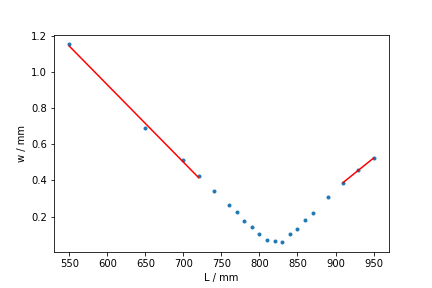
\includegraphics[scale = 0.75]{Bilder/Auswertung/gerfithh.png}
    \caption{Strahldurchmesser $w$ aufgetragen in blauen Punkten gegen die Position $L$ für den vertikalen Schnitt durch den Strahl. Dabei ist der lineare Verlauf für Werte weit entgernt von der Strahltaille 
    gut zu erkennen; die zugehörige lineare Regression ist in Rot eingetragen.}
    \label{pic:gerfithh}
\end{figure}
\clearpage
\subsection{Effektive Brennweite der Linse}
\label{subs:f}
Für Gaußsche Strahlen gelten zwar die Gesetze der geometrischen Optik nicht, es kann aber trotzdem eine effektive Brennweite $f_{eff}$ nach 
\begin{equation*}
    \frac{1}{s} + \frac{1}{s'} = \frac{1}{f_{eff}}
\end{equation*}
bestimmt werden. Nimmt man nun an, dass die Strahltaille des Experimentierlasers in der Mitte des Resonators liegt, so gilt für die Strecke zwischen Strahltaille und 
Linse $s$
\begin{align*}
    s &= d_{Linse-Spiegel} + d_{Spiegel-Spiegel} + d_{Spiegel-Resonator} + 0,5 \cdot L_{Resonator} = \\
    &= ((370 - 40) + 201 + (420-50) + 0,5 \cdot 540)\mathrm{mm}.
\end{align*}
Die verwendeten Längen wurden dem Protokoll entnommen. Bei einem Fehler von 5\,mm pro Länge ergibt dies nach Fehlerfortpflanzung einen Fehler von $s_m = 28$\,mm. 
Die Länge $s'$ ist abhängig von der Position der Strahltaille nach der Linse und variiert zwischen senkrechtem und waagerechtem Schnitt durch den Strahl. Für die 
Positionen und Fehler wurden die Werte aus Tab.\ref{tab:M} bis \ref{tab:M3} genommen. Damit ergeben sich
\begin{equation*}
    s'_v = (410 \pm 14)\mathrm{mm} \qquad s'_h = (400 \pm 14)\mathrm{mm}.
\end{equation*}
Aus diesen Werten lassen sich die Werte für $f_{eff}$ berechnen; die dazugehörigen Fehler folgen aus der Fehlerfortpflanzung, wobei folgende Beziehung verwendet wurde:
\begin{equation*}
    \partial_{s^{(|)}}f_{eff} = \frac{f_{eff}^2}{s^{(|)2}}
\end{equation*}
Die effektiven Brennweiten sind
\begin{equation*}
    f_{eff,v} = (303 \pm 13)\,\mathrm{mm}\qquad\mathrm{und }f_{eff,h}=(298 \pm 13)\,\mathrm{mm}
\end{equation*}
Bildet man den Mittelwert, so hat die Linse unseren Berechnungen nach eine effektive Brennweite von
\begin{equation*}
    \textcolor{red}{f_{eff} = (301 \pm 9)\, \mathrm{mm}}
\end{equation*}
Dieses Ergebnis stimmt auch gut mit der Angabe auf der Linse selbst überein; deshalb kann es als sinnvoll angesehen werden.

\subsection{Strahltaillen}
\subsubsection*{Im Resonator}
Die Stahltaille im Resonator ergibt sich nach 
\begin{equation*}
    w_{00} = \sqrt{\frac{\lambda L}{\pi}} \cdot \biggl(\frac{(1-g^2)}{4(1-g)^2}\biggl)^{0,25},
\end{equation*}
wobei $L$ die Resonatorlänge und $g = 1 - \frac{L}{R}$ der Spiegelparameter mit Spiegelkrümmungsradius $R$ ist. Ferner wurde benutzt, dass $R$ und somit $g$ für beide Spiegel 
gleich sind(\cite{TUB2018}, S.8). 
Für die Fehlerfortpflanzung wurden dabei die folgenden Ableitungen verwendet:
\begin{align*}
    \partial_Lw_{00}  &= \frac{w_{00}}{2L}\\
    \partial_gw_{00} &= w_{00} \frac{1 - g(1-g)}{2(1-g)(1-g^2)}
\end{align*}
Die Fehler für $L$ und damit für $g$ sind die aus der Messung der Resonatorlänge. Insgesamt ergibt sich die Strahltaille zu
\begin{equation*}
    \textcolor{red}{w_{00} = (224,0 \pm 1,5)\,\mu\mathrm{m}}
\end{equation*}

\subsubsection*{Hinter der Linse, berechnet}
Ausgehend von der berechneten Strahltaille im Resonator ergibt sich die Strahltaille hinter der Linse nach 
\begin{equation*}
    w_0 = w_{00}\,\sqrt{\frac{s'-f}{|s|-f}}. \mathrm{\footnotemark}
\end{equation*}
\footnotetext{\url{https://www.edmundoptics.de/knowledge-center/application-notes/lasers/gaussian-beam-propagation/}, Stand:08.10.21}
Dabei entsprechen die Werte für $s$, $s'$ und $f$ denen aus Abschnitt \ref{subs:f}. Für die Fehlerfortpflanzung wurden folgende partielle Ableitungen verwendet: 
\begin{align*}
    \partial_{w_{00}}w_0 &= \frac{w_0}{w_{00}}\\
    \partial_{s^{(|)}}w_{0} &= \mp \frac{w_0}{2(s^{(|)}-f)}
\end{align*}
Damit ergeben sich für die berechneten Strahltaillen für den vertikalen bzw. horizontalen Schnitt des Strahls die Werte 
\begin{equation*}
    \textcolor{red}{w_{0,v} = (78 \pm 7)\,\mu\mathrm{m} \qquad w_{0,h} = (77 \pm 7)\,\mu\mathrm{m}}.
\end{equation*}
Vergleicht man diese mit dem gemessenen Werten für $w_0$ in Tab.\ref{tab:M} und \ref{tab:M1} ($w_{0,v}$ = (60,9  $\pm$ 2)\,$\mu$m, $w_{0,h}$ = (59,3  $\pm$ 4)\,$\mu$m), so ist festzustellen, 
dass die Werte in der selben Größenordnung liegen. Allerdings sind die berechneten Werte um etwa den Faktor 1,3 zu groß und die Abweichung lässt sich auch nicht alleine durch 
die berechneten Fehler erklären. Möglicherweise liegt der Fehler in dem nicht idealen Versuchsaufbau oder es wurden in der Berechnung weitere Faktoren vernachlässigt (z.B. 
könnte die Strahltaille nicht exakt in der Mitte des Resonators liegen oder noch wahrscheinlicher die Strahltaille wurde nicht an der exakten Position hinter der Linse 
bestimmt).

\subsection{Intensität im Fokus}
Die Intensität eines Gaußstrahls lässt sich schreiben als 
\begin{equation*}
    %I = I_0 \exp(\frac{-2r^2}{w^2}), \mathrm{\footnotemark}
    I = \frac{2P}{\pi w^2} \exp(\frac{-2r^2}{w^2}), \mathrm{\footnotemark}
\end{equation*}
\footnotetext{\url{https://www.edmundoptics.de/knowledge-center/application-notes/lasers/gaussian-beam-propagation/}, Stand:08.10.21}
wobei $r$ der radiale Abstand zur Stahlmitte und $P$ die Leistung des Lasers ist. Die Leistung innerhalb einer Kreisscheibe mit Radius $R$ berechnet sich nach 
\begin{align*}
    P(R) &= \iint I(r) dA = \frac{2P}{\pi w^2} \int_0^{2\pi} \int_0^R \exp(\frac{-2r^2}{w^2})r\, d\phi dr = \\
    &= \frac{4P}{w^2} [-\frac{w^2}{4}\exp(\frac{-2r^2}{w^2})]_0^R \\
    &= P (1-\exp(\frac{-2R^2}{w^2}))\\
    &= P(1-e^{-2}),
\end{align*}
wobei im letzten Schritt für $R$ der Strahldurchmesser $w$ eingesetzt wurde. Im Fokus gilt $w = w_0$ damit folgt für die Leistung pro Fläche (=Intensität)
\begin{equation*}
    \frac{P}{A} = I_{fok} = \frac{P(1-e^{-2})}{w^2\pi} = \frac{P(1-e^{-2})}{w_0^2\pi}
\end{equation*}
Und mit $P =$1\,mW, der Ableitung für die Fehlerfortpflanzung 
\begin{equation*}
    \partial_{w_0}I = \frac{2I}{w_0}s_{w_0}
\end{equation*}
und dem Wert für die Strahltaille aus Tab.\ref{tab:M} ergibt sich ein Wert von 
\begin{equation*}
    \textcolor{red}{I_{fok} = (73,0 \pm 1,0)\,\frac{\mathrm{kW}}{\mathrm{m^2}}}
\end{equation*}
(für den horizontalen und vertikalen Schnitt des Strahls sind die Taillen fast identisch; zur Abschätzung der gesamten 
Strahltaille wurde der größere von beiden gewählt).
